\chapter{Signature of the Signal}
\label{cha:sig}

As discussed in section~\ref{sec:anamodel}, the model used in the analysis is $R$-parity violating supersymmetry. In particular, single coupling dominance for the lepton number violating coupling $\lambda^\prime_{211}$ is assumed. With a two quark initial state, the production of sleptons inevitably dominates other constellations. Taking into consideration how small the values of $\lambda^\prime_{211}$ have to be (Cf.~fig.~\ref{fig:auterrpv}~\&~\ref{fig:2011rpv}), the primary decay modes for the slepton will be the $R$-parity \textit{conserving} $\nu + \tilde{\chi}^\pm$ or $\mu + \tilde{\chi}^0$ processes. While the decay width for these modes are independent of $\lambda^\prime_{211}$ coupling, the competing $R$-parity \textit{violating} dijet decay channel depends on it. With strict bounds of at least $\lambda^\prime_{211} < 0.01$, the decay width of the $R$-parity conserving gaugino decay modes are two orders of magnitude larger than the $R$-parity violating one. As a result, they total decay width is mostly independent of the $\lambda^\prime_{211}$ parameter. Since the production cross section for smuons $\sigma_{\tilde{\mu}}$ and sneutrinos $\sigma_{\tilde{\nu}}$ scales quadratically with the matrix element, it is proportional to $\lambda^{\prime\:2}_{211}$. Consequently, the overall cross sections $\sigma(qq' \rightarrow \tilde{\mu} \rightarrow \mu\tilde{\chi}^0)$ and $\sigma(qq' \rightarrow \tilde{\nu} \rightarrow \nu\tilde{\chi}^\pm)$ also have a quadratic dependence on $\lambda^\prime_{211}$ for values lower than $0.01$.

The lightest neutralino is assumed to be the lightest supersymmetric particle (\textbf{LSP}), which is not considered to be stable in this analysis. Production and decay of both the chargino and heavier neutralinos can lead to additional jets or leptons, but will eventually lead to the lightest neutralino through the $R$-parity conserving modes\footnote{The details of the decay modes depend on the mass hierarchy determined by the RPV cMSSM model parameters. The dependence on the universal mass parameters will be studied in the next section.} (Fig.~\ref{fig:resosmusneu}). 

\begin{figure}[ht!]
  \centering
  \begin{subfigure}[b]{0.495\textwidth}
    \centering
    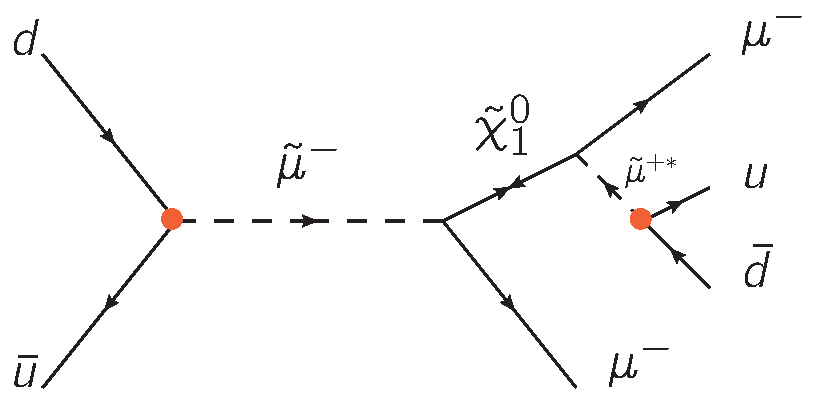
\includegraphics[width=\textwidth]{plots/rpv-resonant-smuon-samesign-mumuqq.pdf}
    \caption{\label{fig:ressmu}}
  \end{subfigure}
  \begin{subfigure}[b]{0.495\textwidth}
    \centering
    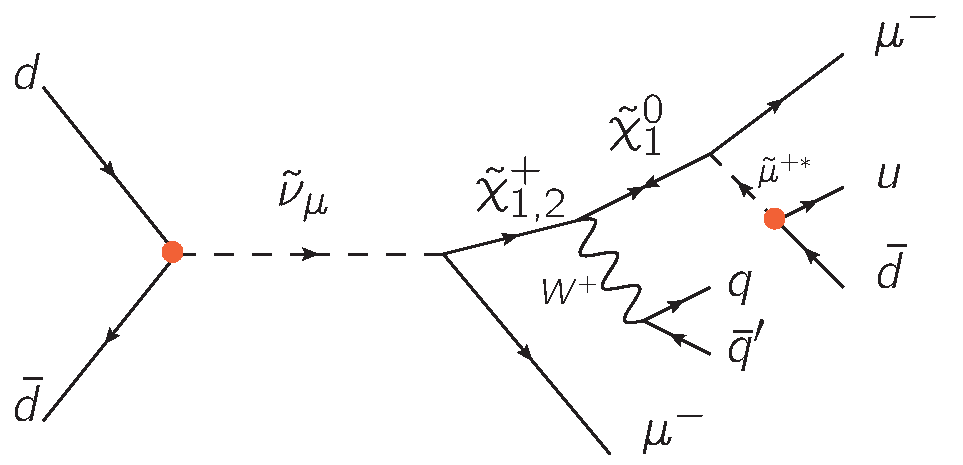
\includegraphics[width=\textwidth]{plots/rpv-resonant-sneutrino-chargino-mumuqq.pdf}
    \caption{\label{fig:ressneu}}
  \end{subfigure}
  \caption{Resonant production of a smuon~(\ref{fig:ressmu}) and a sneutrino~(\ref{fig:ressneu}) in $R$-parity violating supersymmetry. Shown are the most simple Feynman graphs leading to the two muon, two jets final state. The lepton number violating vertices are marked in red.}
  \label{fig:resosmusneu}
\end{figure}

Since it is the LSP, it can only decay through the $\lambda^\prime_{211}$ coupling via a virtual smuon or sneutrino. It should also be noted that the lifetime of the LSP depends on the coupling strength. For values $\lambda^\prime_{211} > 10^{-6}$, the decay will be perceived as ``prompt'' by the detector. This means that both muons should originate from the same (primary) vertex. The decay of the LSP subsequently adds two jets, as well as either a muon or neutrino. With missing transverse energy from neutrinos being significantly less attractive than muon signatures, these final states are neglected. 

This leaves two jets and a number of muons, ranging from zero to two, in every decay. Considering the production rates for the relevant backgrounds, one can see that two compositions are disfavoured. Colliding two hadrons yields a high amount of jets in every event, making the pure dijet channel without any muon the least promising. The very high $W + \text{jets}$ background would interfere with a single muon and two jets search, leaving only the two muons, two jets option. Even here there are significant backgrounds to tackle, primarily the Drell-Yan process.

Taking a look at the simplest Feynman graphs for resonant smuon and sneutrino production and decay at the LHC (Fig.~\ref{fig:resosmusneu}), one will notice a very useful attribute of their decay products. The electric charge of both muons are equally as likely to have the same sign as the opposite sign. This is due to the neutralino being a Majorana particle. Keeping the initial state of two protons in mind, primarily the ratio of $u$ to $d$-quarks, the likelihood of positively charged muons is roughly twice the one for negatively charged ones. Since most Standard Model backgrounds are able to produce two opposite, but not two same sign muons, this feature of RPV supersymmetry can be exploited to discriminate against them. Major backgrounds, such as the aforementioned Drell-Yan processes or the production of top quark pairs, can be greatly reduced, enabling searches for new physics with low cross sections.


\section{Monte Carlo Study}
\label{sec:mcstudy}

As Monte Carlo (\textbf{MC}) simulations are used for comparison to the measured data, the simulation of the signal for the $7\,\text{TeV}$ CMS data taking period~\cite{2011rpv} can be used to derive further information about the signature. The production process of such a simulation will be outlined in section~\ref{sec:signal-sim}. Using the RPV supersymmetry model explained in section~\ref{sec:anamodel}, a grid of simulated signal points with $50\,\text{k}$ events each has been generated. While the scalar sparticle mass parameter $m_0$ runs from $100$ to $2000\,\text{GeV}$ in steps of $100\,\text{GeV}$ and the mass parametr of fermionic sparticles $m_{1/2}$ runs from $50$ to $1000\,\text{GeV}$ in steps of $50\,\text{GeV}$, the remaining model parameters have the following fixed values:

\begin{equation*}
  A_0 = 0, \quad \tan{\beta} = 20, \quad \text{sgn}\,\mu = +1, \quad \lambda^\prime_{211} = 0.01
\end{equation*}

The cMSSM parameter values are inspired by the low mass benchmark points of CMS~\cite{cmssusybenchmarkpoints} and are chosen such, that small variations have little impact on the sparticle mass hierarchy and consequently the signature. Quantifying these ``small variations'' is difficult, as the sparticle masses do not just depend on one parameter. In general, changes of a few $100\,\text{GeV}$ for $A_0$, around $10$ for $\tan{\beta}$ and any sign of $\mu$ will result in the same mass hierarchy. The value of the $R$-parity violating coupling $\lambda^\prime_{211}$ is based on a rough estimate for the sensitvity of hadron colliders~\cite{rpvimpl}. Because certain regions (low $m_{1/2}$, high $m_0$) in this parameter space lead to unphysical phenomena such as non-converging renormalization group equations, tachyonic solutions or no electroweak symmetry breaking, they are not being simulated. Excluding these points in the grid leaves an overall amount of $354$ simulated phase space points (Cf.~fig.~\ref{fig:sigeff}). \\

Various decay scenarios are being investigated in this grid to determine their respective contribution to the signal signature. Two cases are considered. In the first one at least two muons and two jets are required (\textbf{MU2J2}). This yields signal events, but not all of them pass all analysis requirements. Only the second one demands all analysis requirements (from 2011~\cite{2011rpv}) to be met (\textbf{ANA}). Major differences between the two are the same sign charge requirement and isolation criteria for muons. While it is important to know that the latter is tighter than the first, the details of all the requirements will be discussed in-depth in the event selection\footnote{Although the event selection will concern itself with the 2012 requirements, they are comparable to the ones used in 2011.} (Cha.~\ref{cha:eventsel}). Comparing both types of cases gives an idea of the effect of the analysis requirements on the signal.

To determine the overall efficiency of selecting signal events, the MU2J2 and ANA cases without any specific decay scenario are shown in figure~\ref{fig:sigeff}.

\begin{figure}[ht!]
  \centering
  \begin{subfigure}[b]{0.495\textwidth}
    \centering
    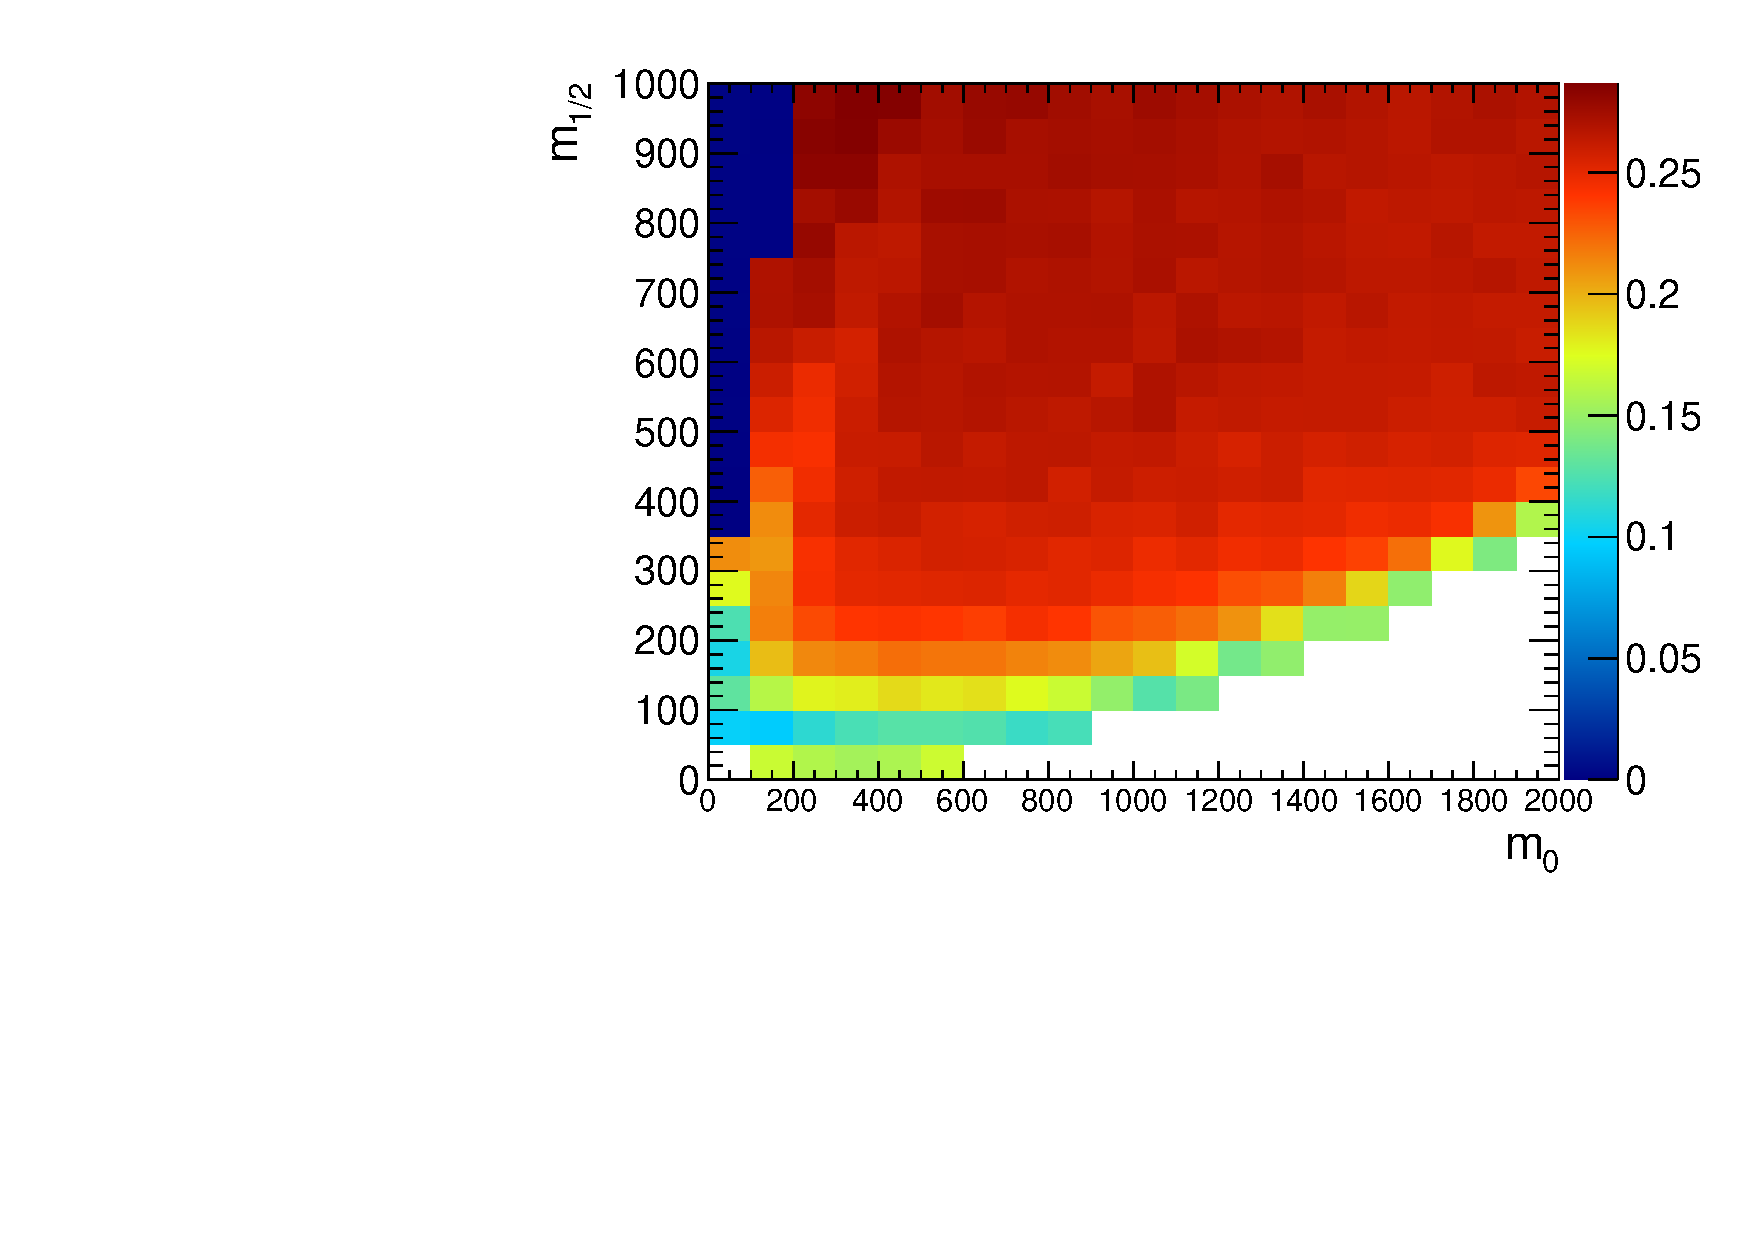
\includegraphics[width=\textwidth]{plots/hSignalRatio.pdf}
    \caption{\label{fig:sig}}
  \end{subfigure}
  \begin{subfigure}[b]{0.495\textwidth}
    \centering
    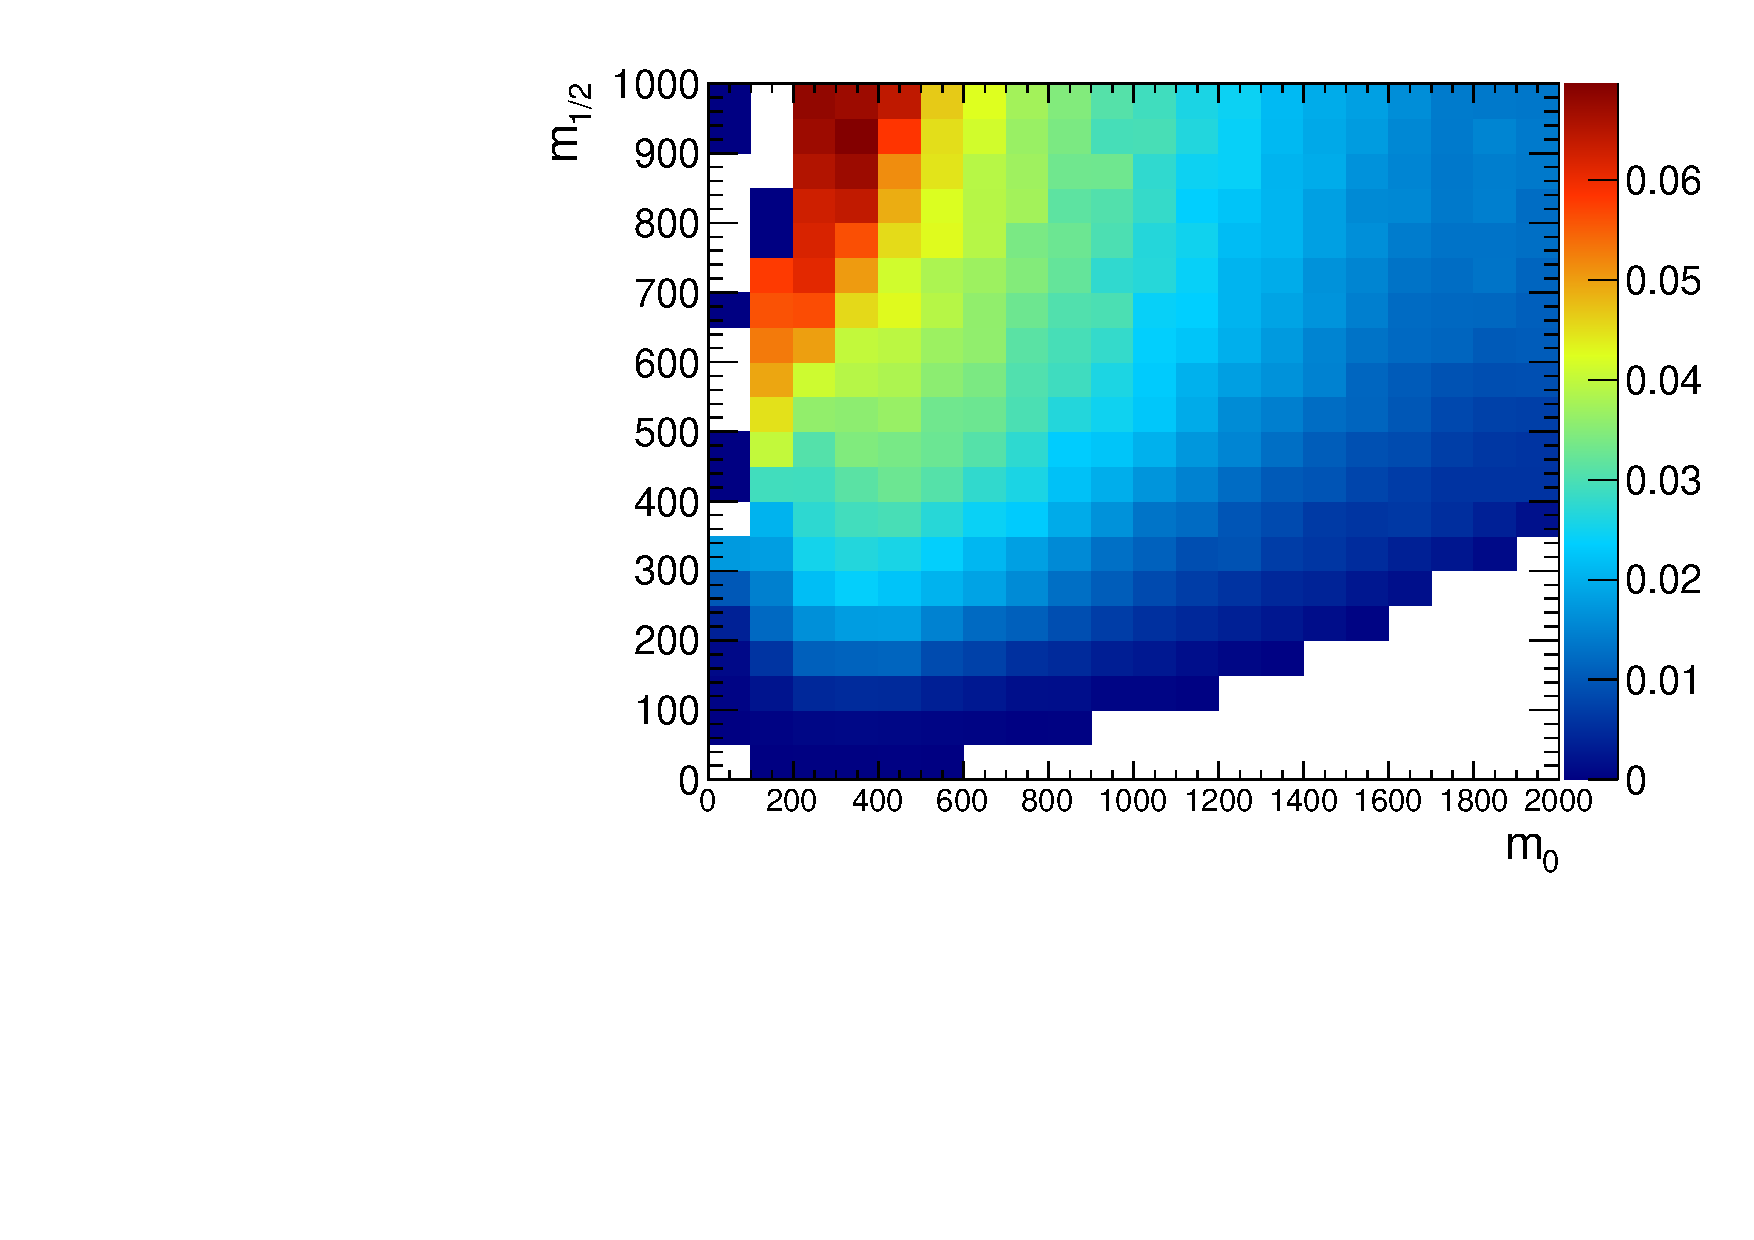
\includegraphics[width=\textwidth]{plots/hCutSignalRatio.pdf}
    \caption{\label{fig:cutsig}}
  \end{subfigure}
  \caption{Efficiency of selecting signal events in the MU2J2~(\ref{fig:sig}) and the ANA case~(\ref{fig:cutsig}). Each bin represents a Monte-Carlo simulation of a RPV supersymmetry point normalized to the generated number of events.}
  \label{fig:sigeff}
\end{figure}

\noindent Each bin shows the number of events meeting the requirements, normalized to the generated number of events. The white bins contain no events. This is either because no events passed the requirements, or they are within the previously mentioned low $m_{1/2}$, high $m_0$ parameter region with unphysical results. For high $m_{1/2}$, but low $m_0$ there are also disproportionally few events. The reason for this disparity lies within the supersymmetric mass spectrum. The lightest supersymmetric particle changes from the lightest neutralino to the stau $\tilde{\tau}$. As a result, the decay chains are altered, therefore rendering the analysis requirements insensitive. 

Shifting the focus on the shape of the distribution, one will notice an almost flat efficiency of around $25\,\pct$ above a certain ratio of $m_{1/2}$ to $m_0$ in the MU2J2 case. However, adding the ANA requirements leads to an efficiency decline from the $\sim 6\,\pct$ high $m_{1/2}$, low $m_0$ region to either around or below $1\,\pct$ for increasing $m_0$ and $m_{1/2}$, respectively. A significant portion of the drop in efficiency is expected when using the ANA case. As discussed in the previous section, the additional same sign charge requirement will half the selected amount of events already. Any further requirements will also have a negative impact on the efficiency, with the isolation criteria for the two muons being the main cause for the decline. If the neutralino masses are much lower than the smuon mass, which is roughly the case for ratios of $m_0$ to $m_{1/2}$ upwards of $2$, it will naturally lead to boosted particles in the decay. Should these decay products be too collimated, the isolation criteria will not be met and the event will be discarded. It should be noted that, as a result of different branching ratios in certain phase space regions, different processes can dominate the final state. Consequently the requirements of the ANA case cannot impact the entire phase space equally. Therefore the origin of the decline is always a combination of multiple quantities. \\

By demanding certain amounts of specific particles in a decay chain, it is possible to reconstruct the process of a selected event. This type of requirement will be referred to as an \textit{effective branching ratio} (\textbf{EBR})\footnote{Strictly speaking, these are not branching ratios, as it is a combination of multiple bra
nching ratios and also depends on the production cross section.} To get an overview of the composition of processes leading to the signal signature, the particle count has been varied systematically. To reduce redundancy, only the primary produced sparticle as well as its supersymmetric decay products are used for process identification. Upon reaching the neutralino LSP in the cascade, the decay through the $\lambda^\prime_{211}$ coupling is always identical.

\begin{figure}[ht!]
  \centering
  \begin{subfigure}[b]{0.495\textwidth}
    \centering
    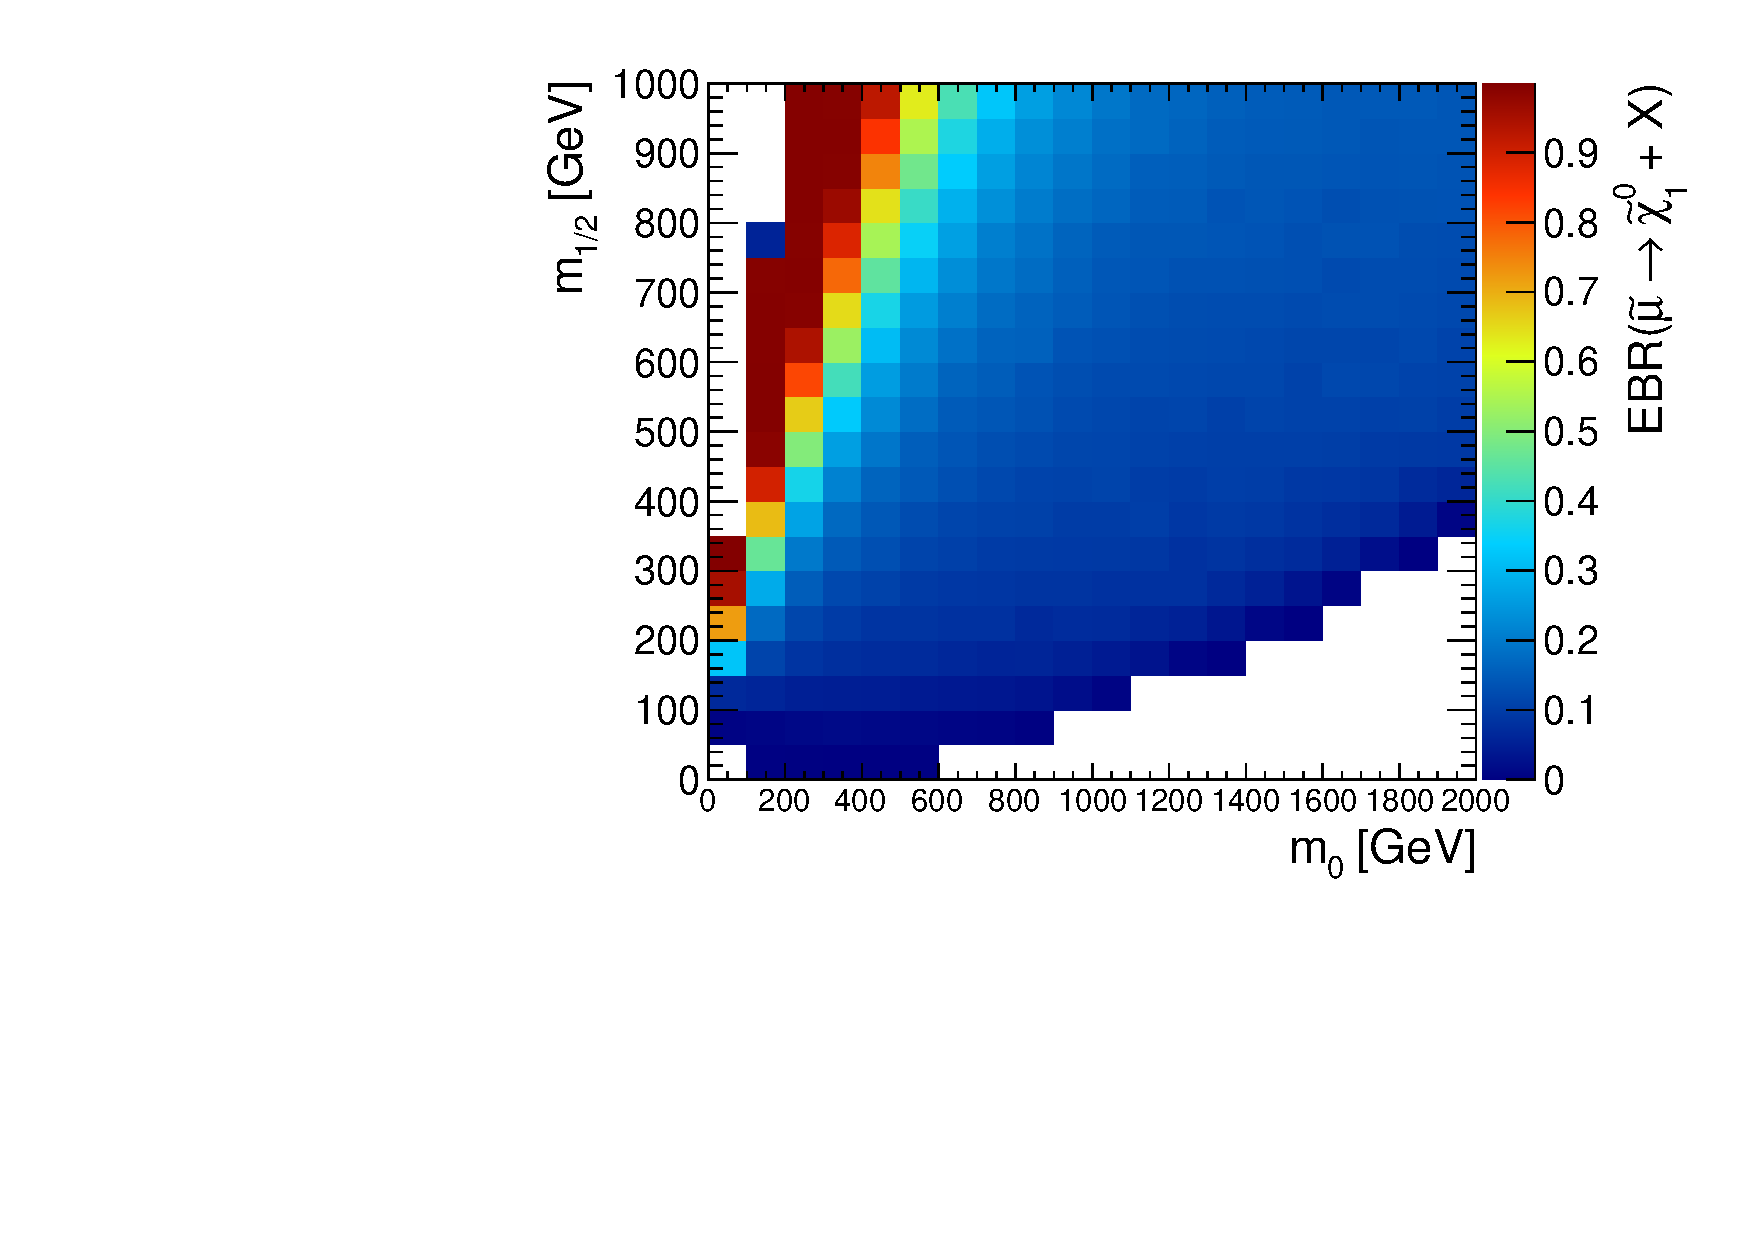
\includegraphics[width=\textwidth]{plots/hX01Ratio.pdf}
    \caption{\label{fig:x01}}
  \end{subfigure}
  \begin{subfigure}[b]{0.495\textwidth}
    \centering
    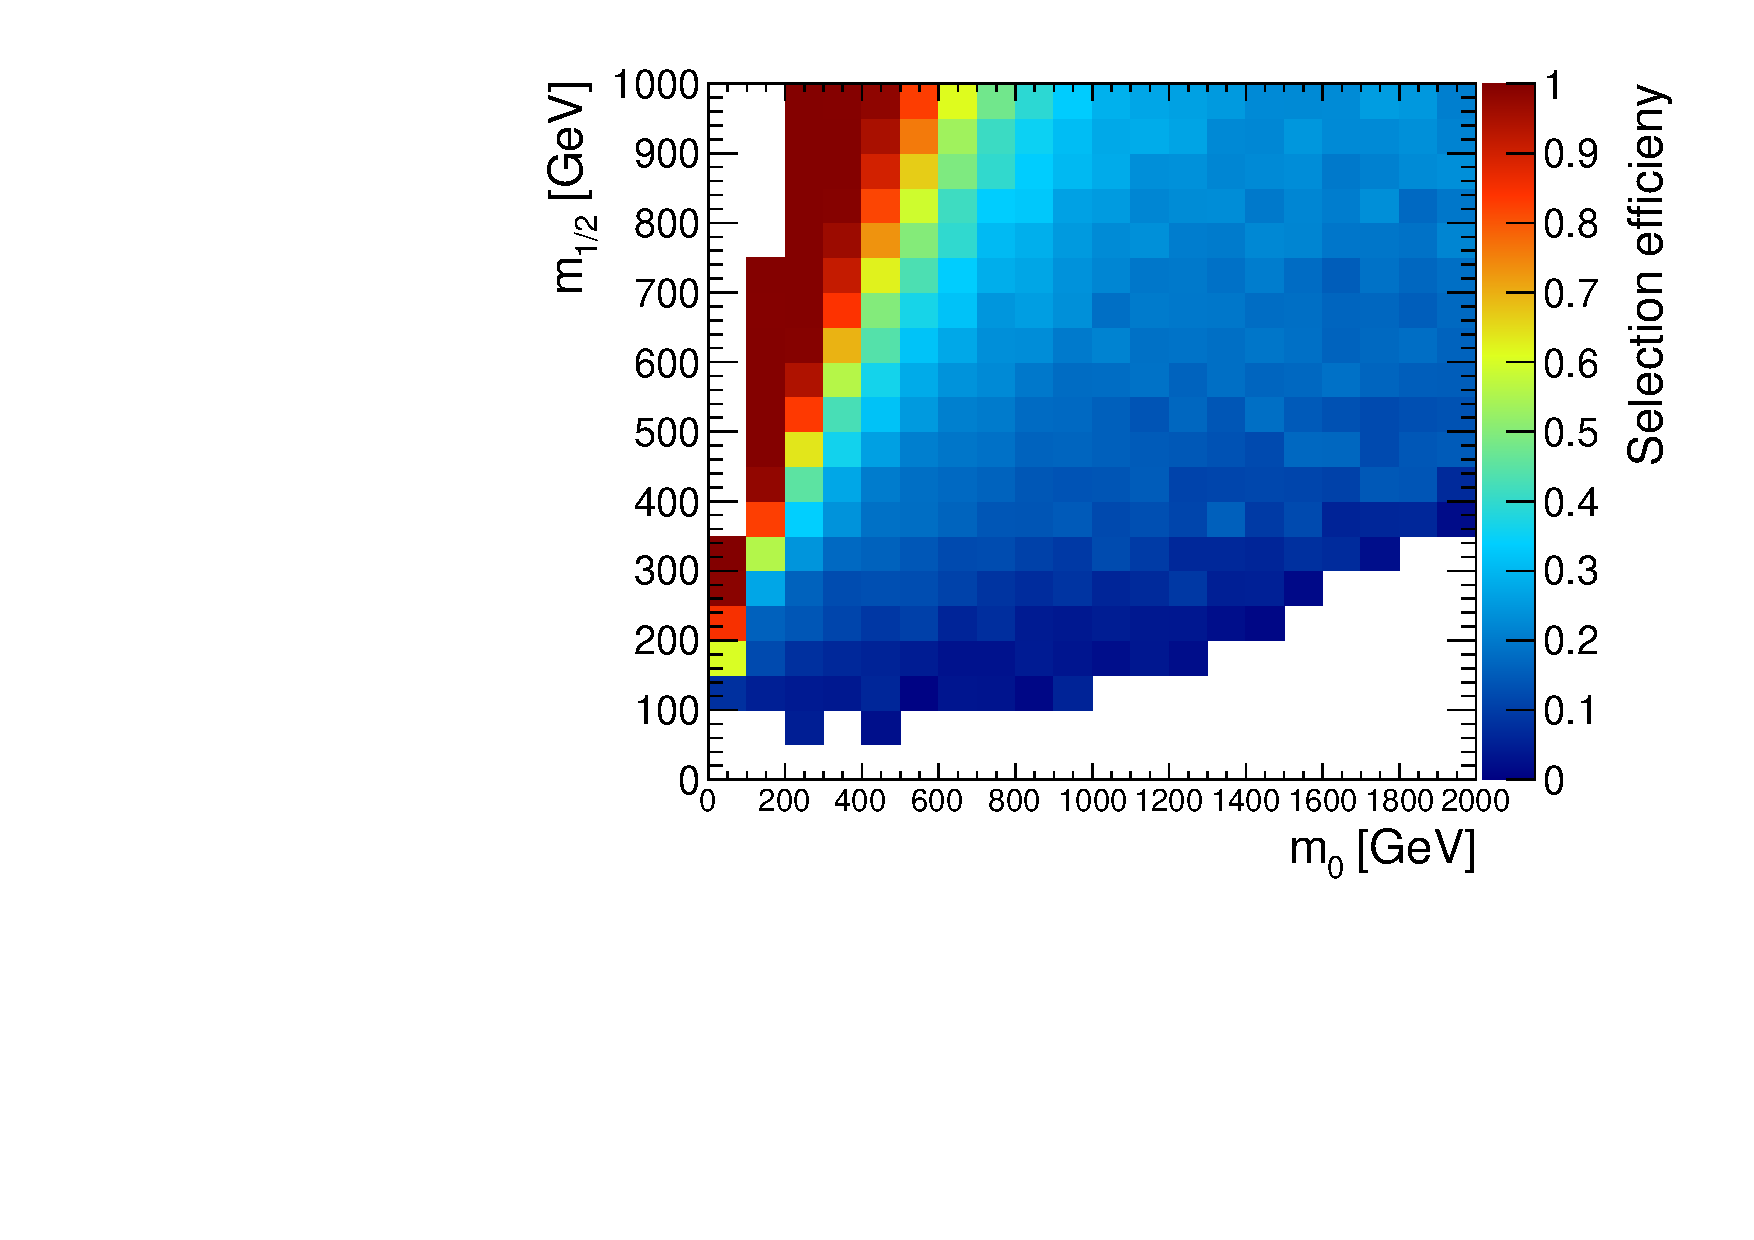
\includegraphics[width=\textwidth]{plots/hCutX01Ratio.pdf}
    \caption{\label{fig:cutx01}}
  \end{subfigure}

  \begin{subfigure}[b]{0.495\textwidth}
    \centering
    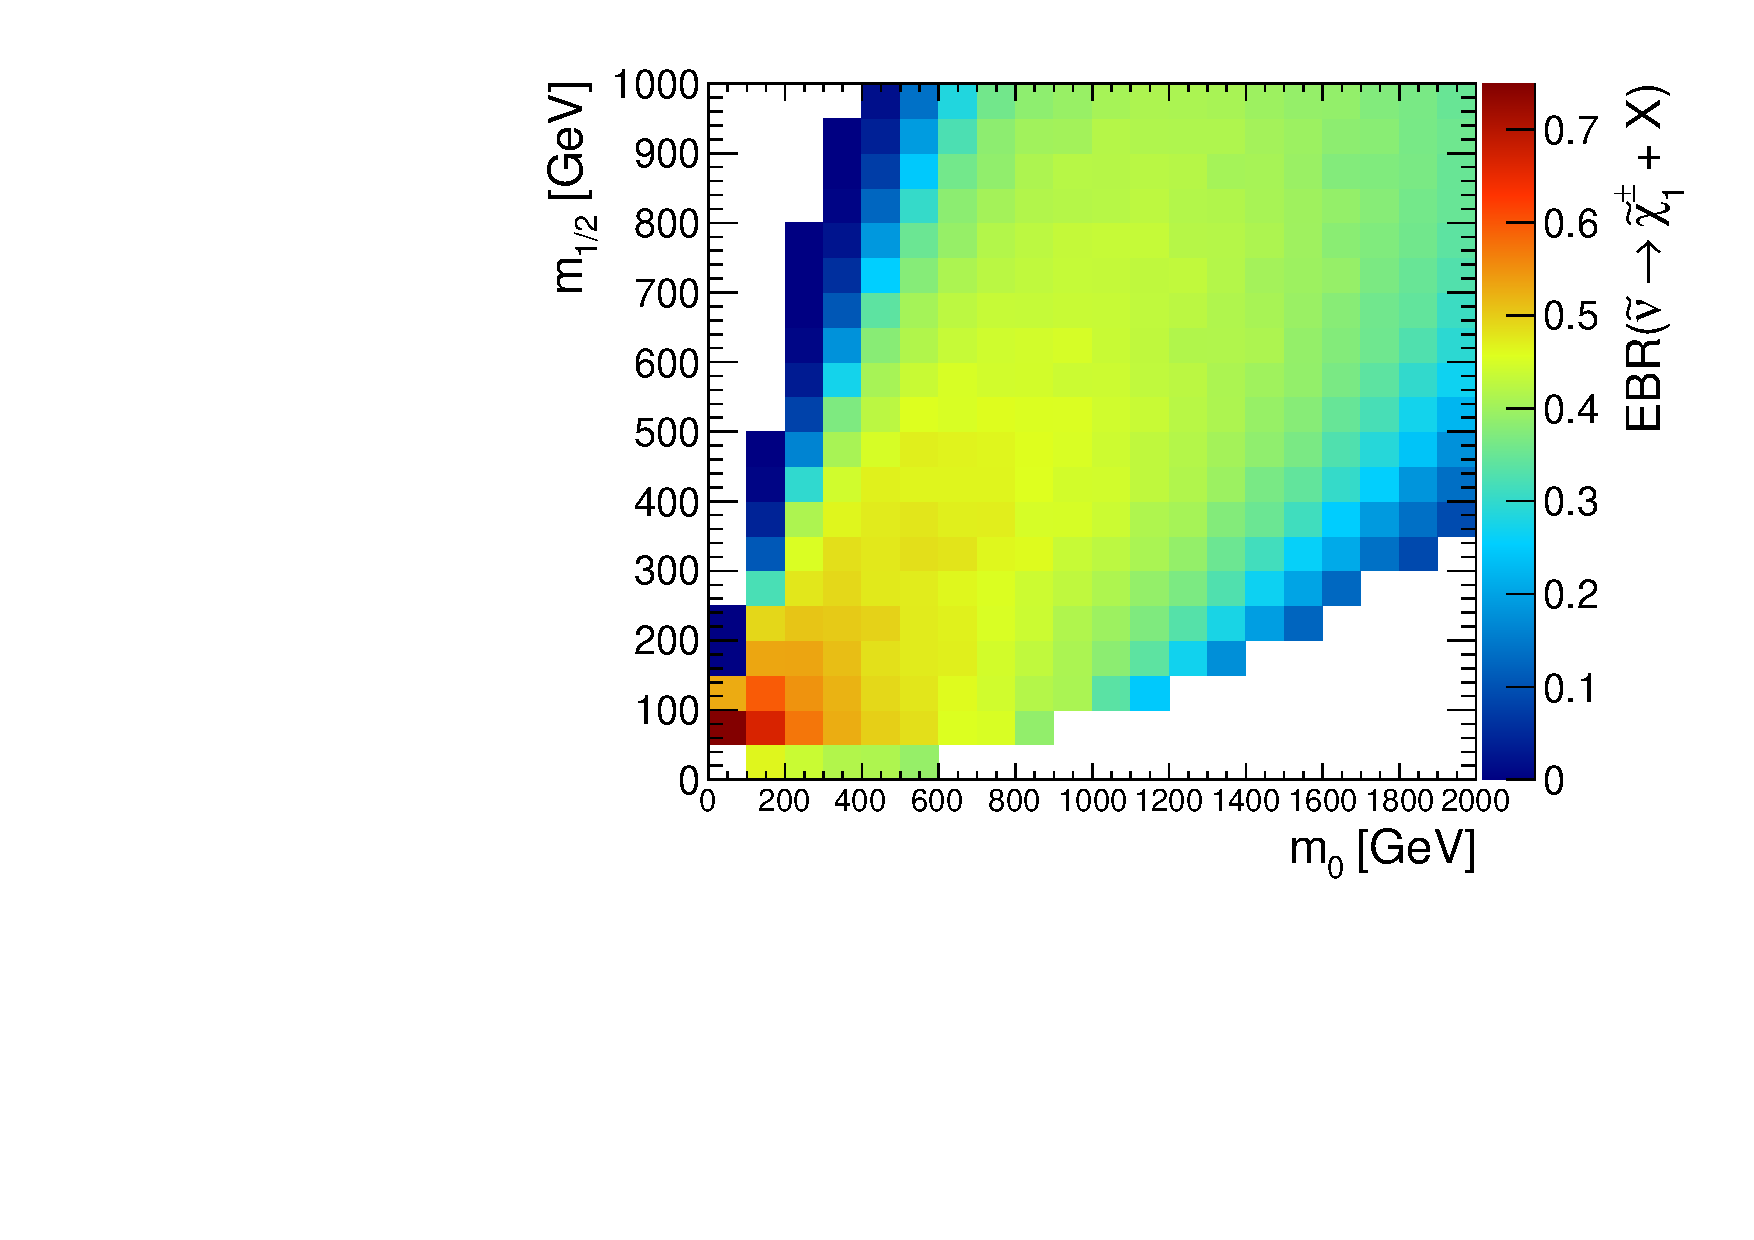
\includegraphics[width=\textwidth]{plots/hXplus1NeutRatio.pdf}
    \caption{\label{fig:xplus1neut}}
  \end{subfigure}
  \begin{subfigure}[b]{0.495\textwidth}
    \centering
    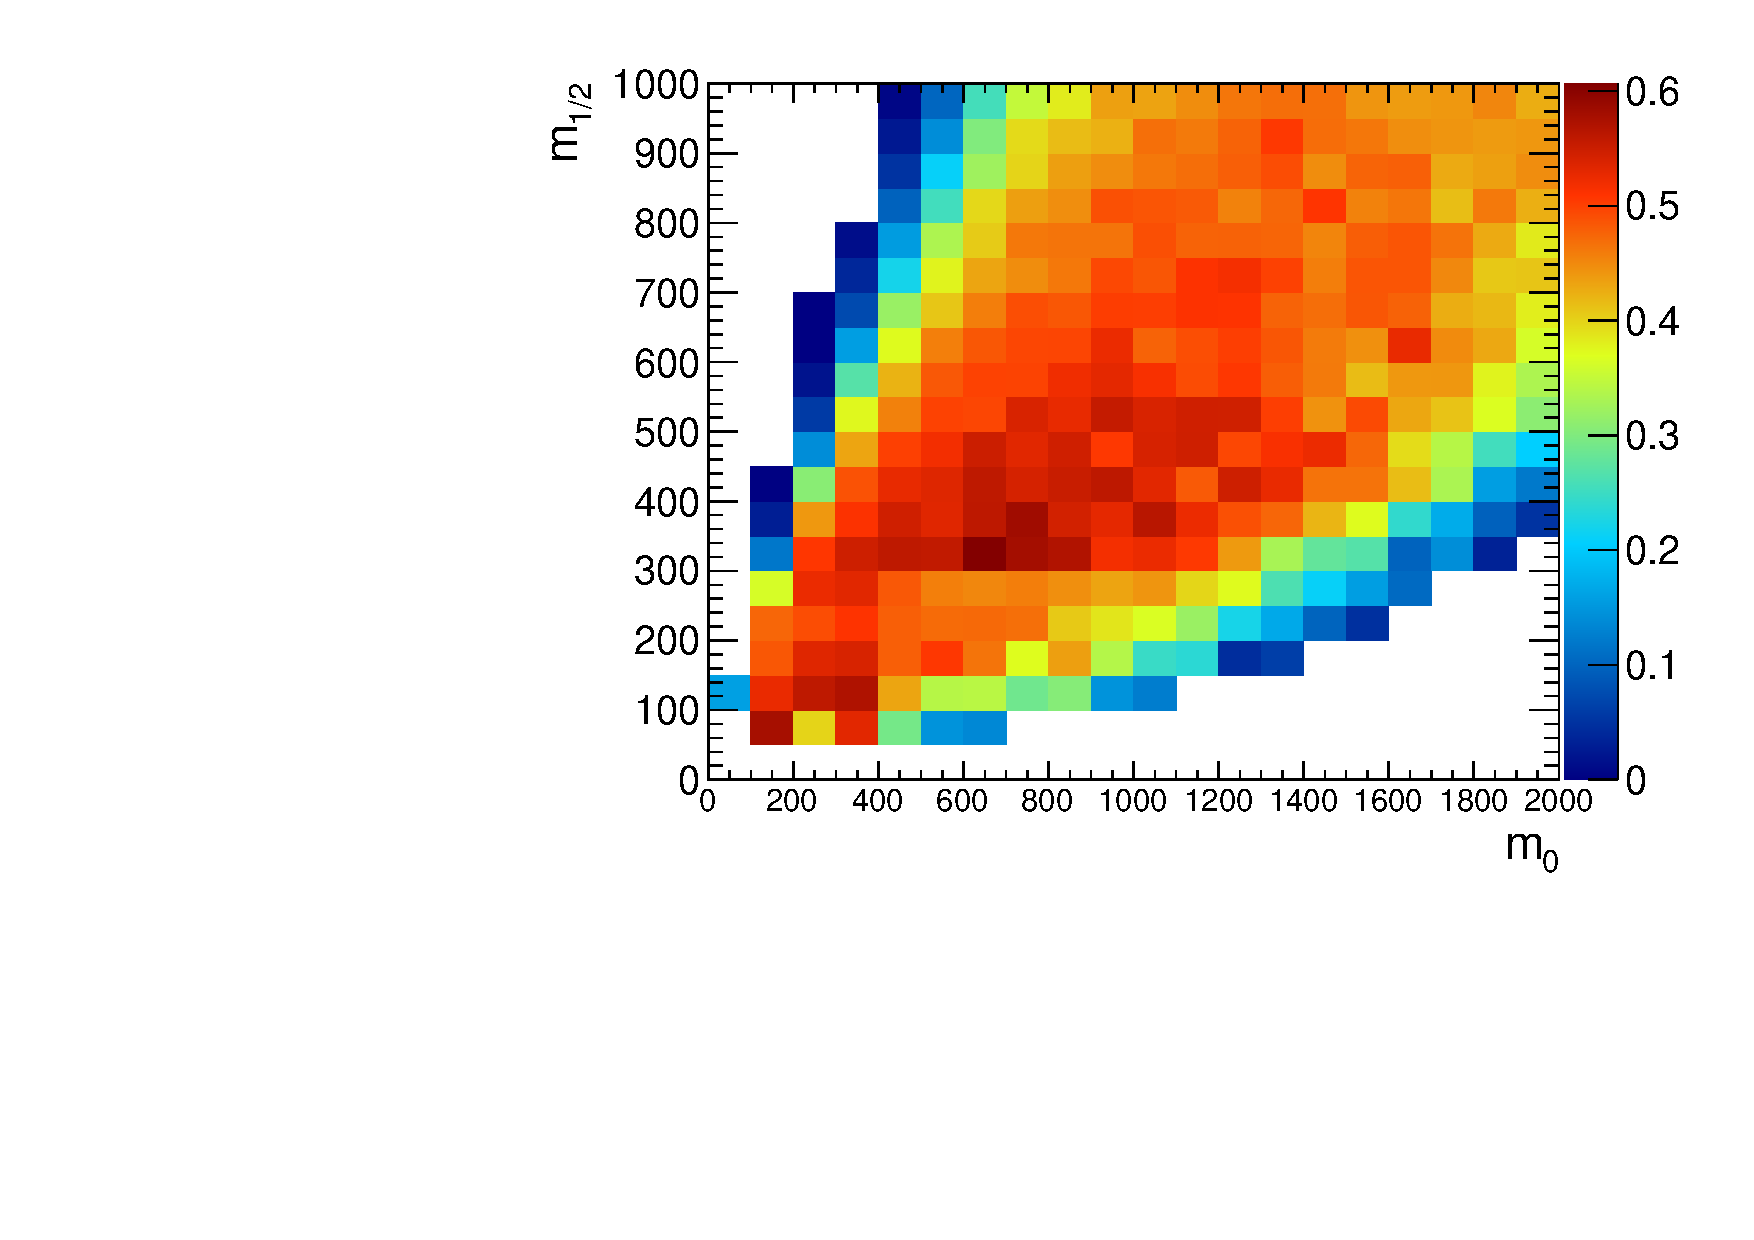
\includegraphics[width=\textwidth]{plots/hCutXplus1NeutRatio.pdf}
    \caption{\label{fig:cutxplus1neut}}
  \end{subfigure}
  \caption{Effective branching ratios of the $\tilde{\mu} \rightarrow \tilde{\chi}^0_1 + X$~(\ref{fig:x01}~\&~\ref{fig:cutx01}) and $\tilde{\nu} \rightarrow \tilde{\chi}^\pm_1 + X$~(\ref{fig:xplus1neut}~\&~\ref{fig:cutxplus1neut}) processes. The EBRs are given by $N_{\text{evt}}(\text{Events including decay products of process}) / N_{\text{evt}}(\text{All events for that bin})$ for each bin of the distribution in figure~\ref{fig:sigeff}. On the left the MU2J2 case is shown, while one can see the ANA case on the right.}
  \label{fig:x01sneuxplusratio}
\end{figure}

\noindent As an example, figure~\ref{fig:x01sneuxplusratio} displays the contributions to the overall selection efficiency from figure~\ref{fig:sigeff} of the $\tilde{\mu} \rightarrow \tilde{\chi}^0_1 + X$ and $\tilde{\nu} \rightarrow \tilde{\chi}^\pm_1 + X$ processes. The effective branching ratio is given by $N_{\text{evt}}(\text{Events including decay products of process}) / N_{\text{evt}}(\text{All events for that bin})$ for the individual bins of the overall selection efficiency.

Combining the ERBs for these two processes already covers roughly $50\pct$ for most of the parameter space. An efficient way to compare all relevant processes at once, is a one dimensional distribution with either of the two universal mass parameters set to a fixed value. Since a larger variation can be observed over the simulated $m_0$ range (Cf. fig.~\ref{fig:sigeff}~\&~\ref{fig:x01sneuxplusratio}), $m_{1/2}$ is kept constant.

\begin{figure}[ht!]
  \centering
  \begin{subfigure}[b]{0.495\textwidth}
    \centering
    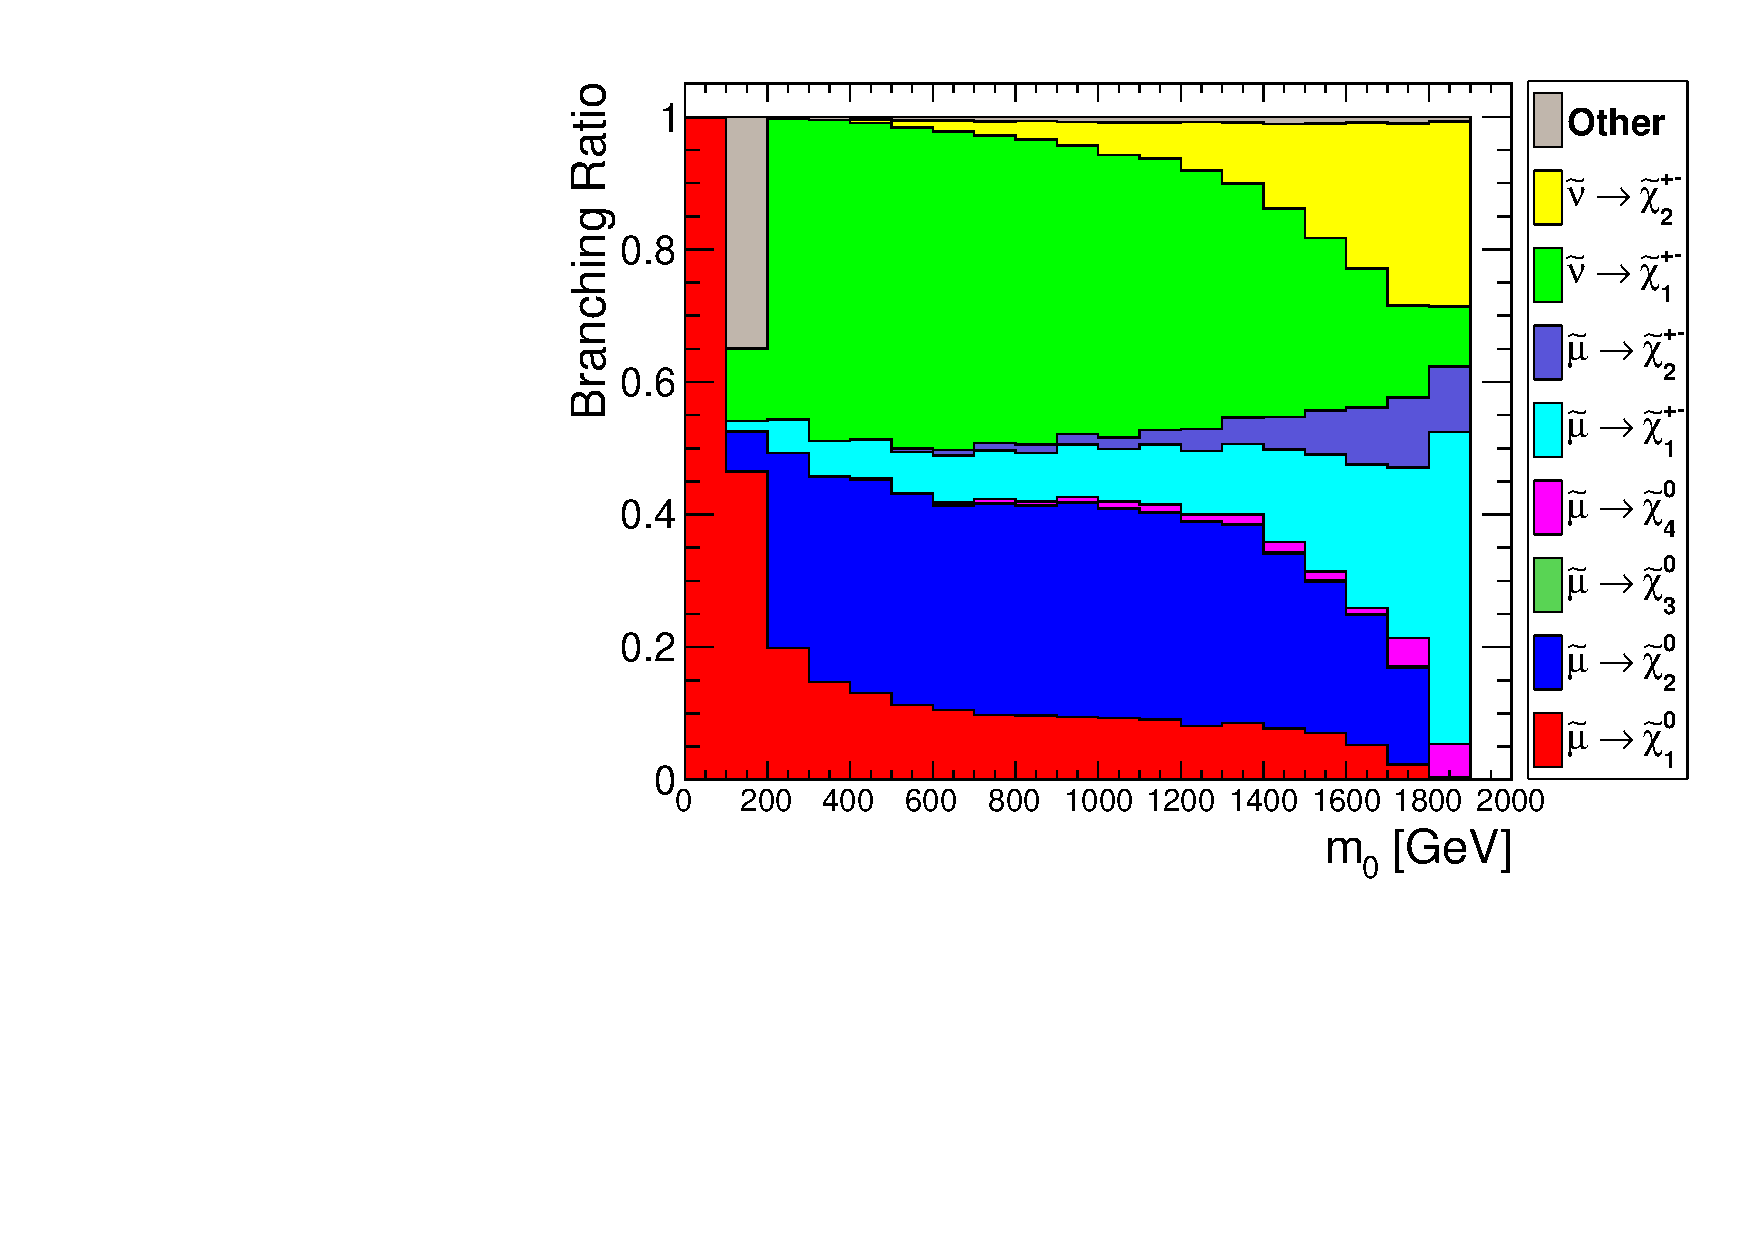
\includegraphics[width=\textwidth]{plots/hCrossRatio350.pdf}
    \caption{$m_{1/2} = 350\,\text{GeV}$\label{fig:crossratio350}}
  \end{subfigure}
  \begin{subfigure}[b]{0.495\textwidth}
    \centering
    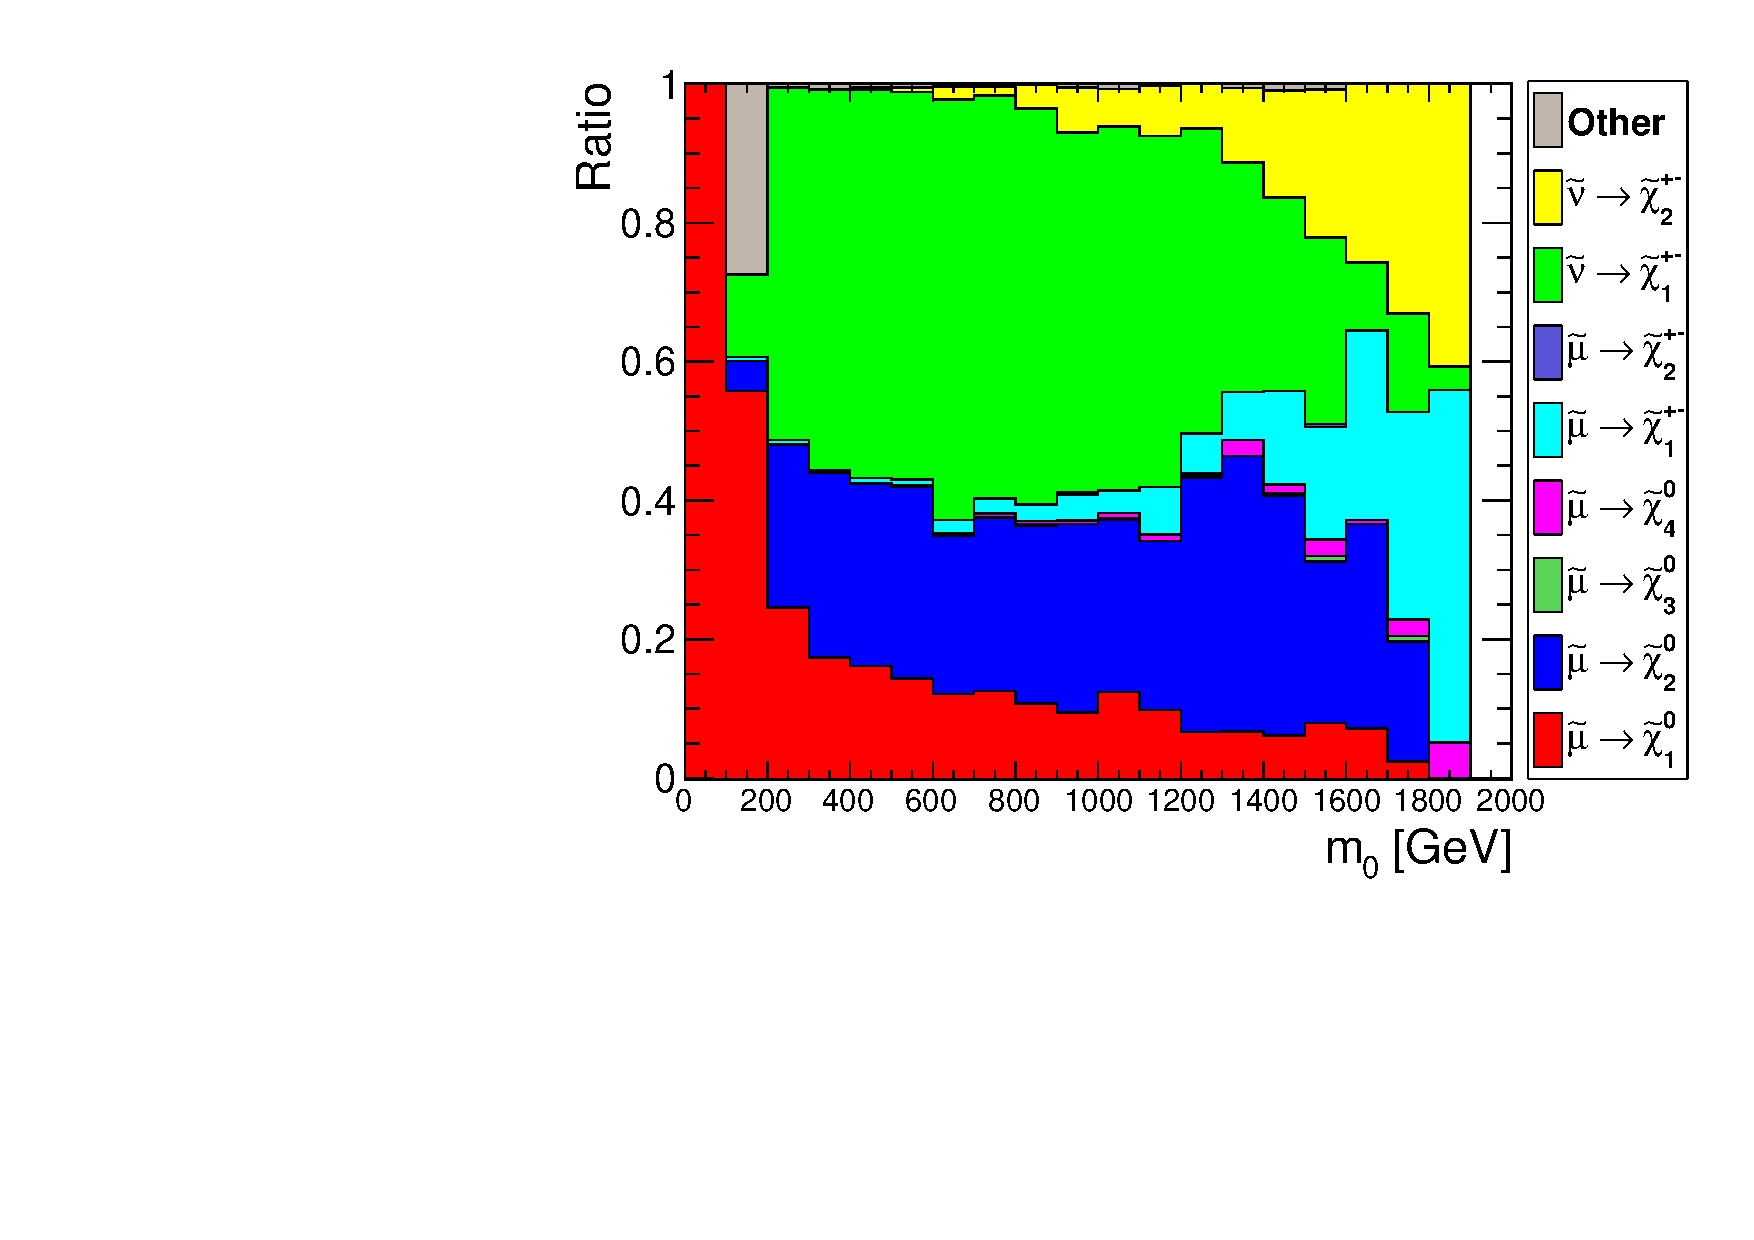
\includegraphics[width=\textwidth]{plots/hCutCrossRatio350.pdf}
    \caption{$m_{1/2} = 350\,\text{GeV}$\label{fig:cutcrossratio350}}
  \end{subfigure}

  \begin{subfigure}[b]{0.495\textwidth}
    \centering
    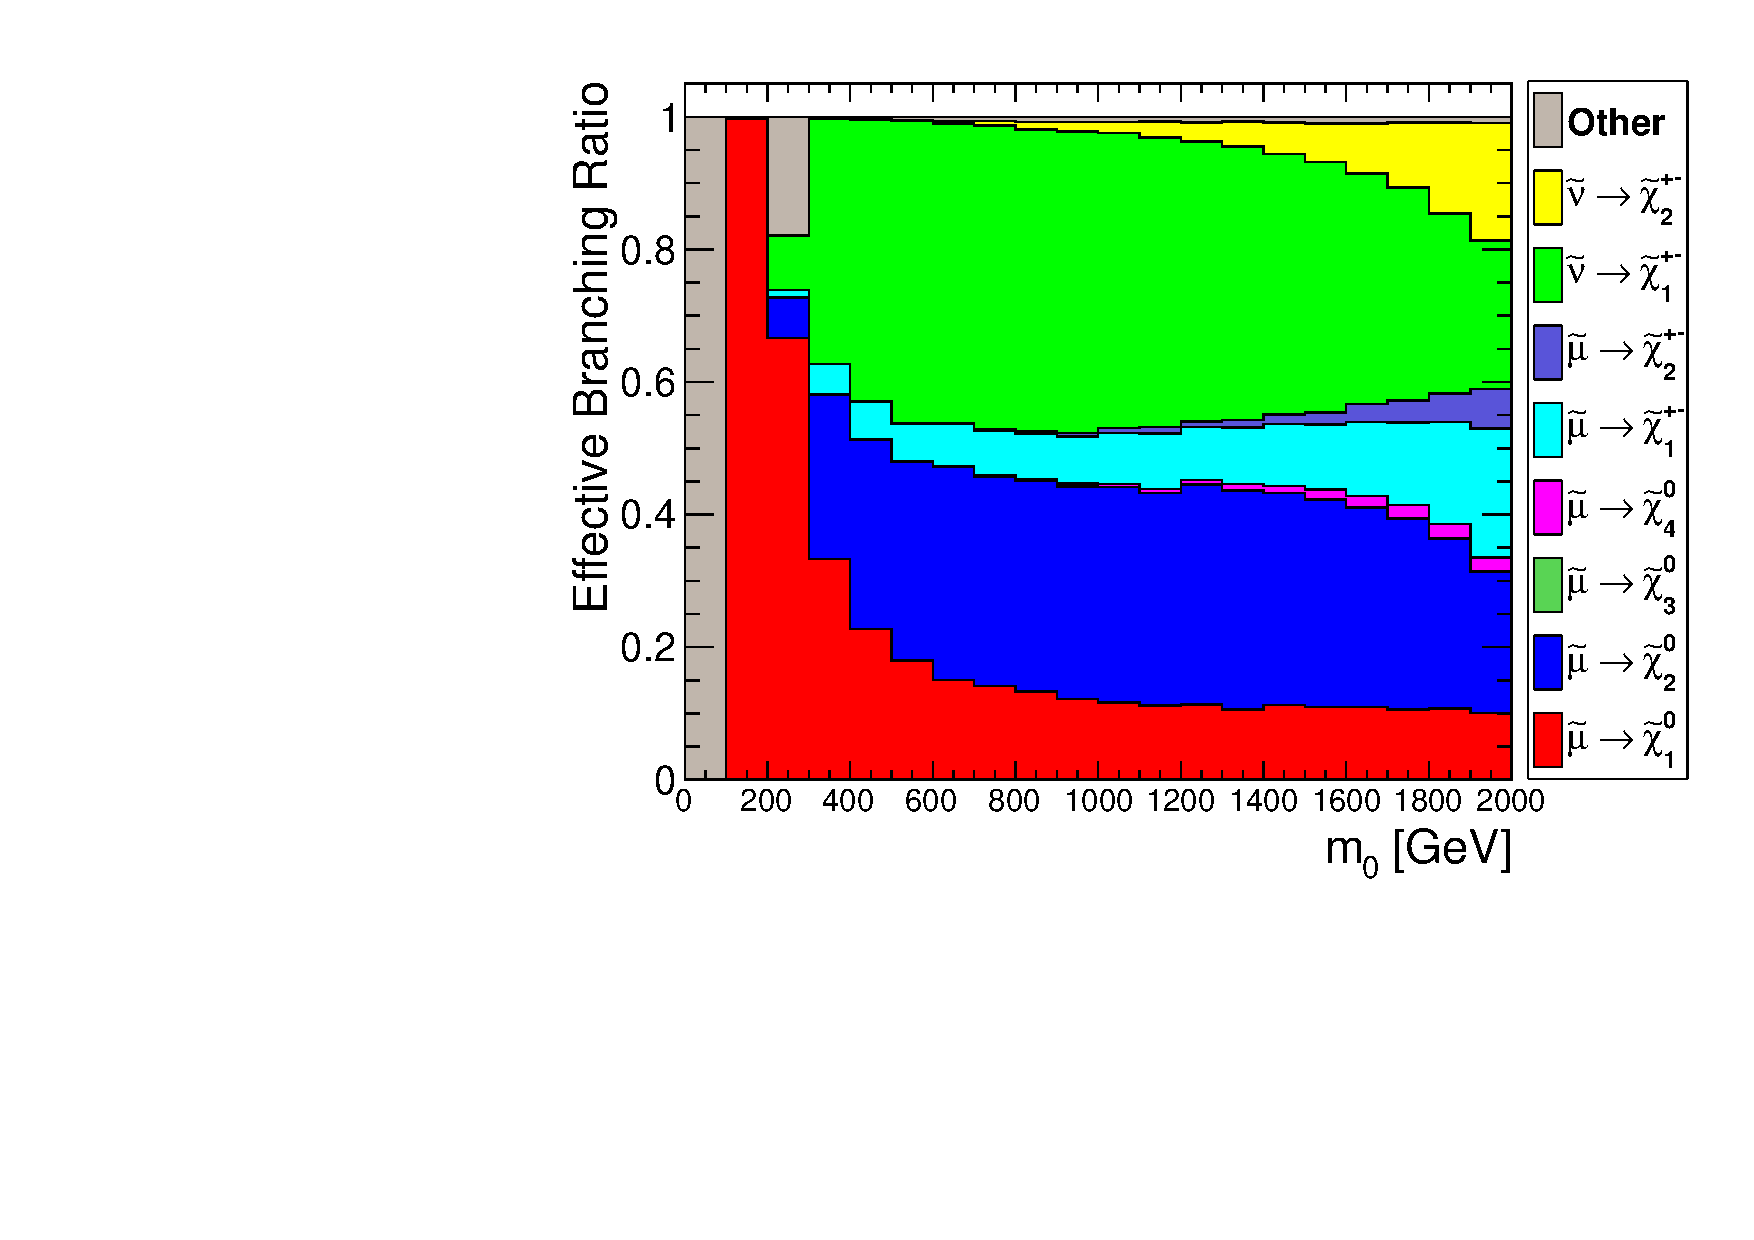
\includegraphics[width=\textwidth]{plots/hCrossRatio550.pdf}
    \caption{$m_{1/2} = 550\,\text{GeV}$\label{fig:crossratio550}}
  \end{subfigure}
  \begin{subfigure}[b]{0.495\textwidth}
    \centering
    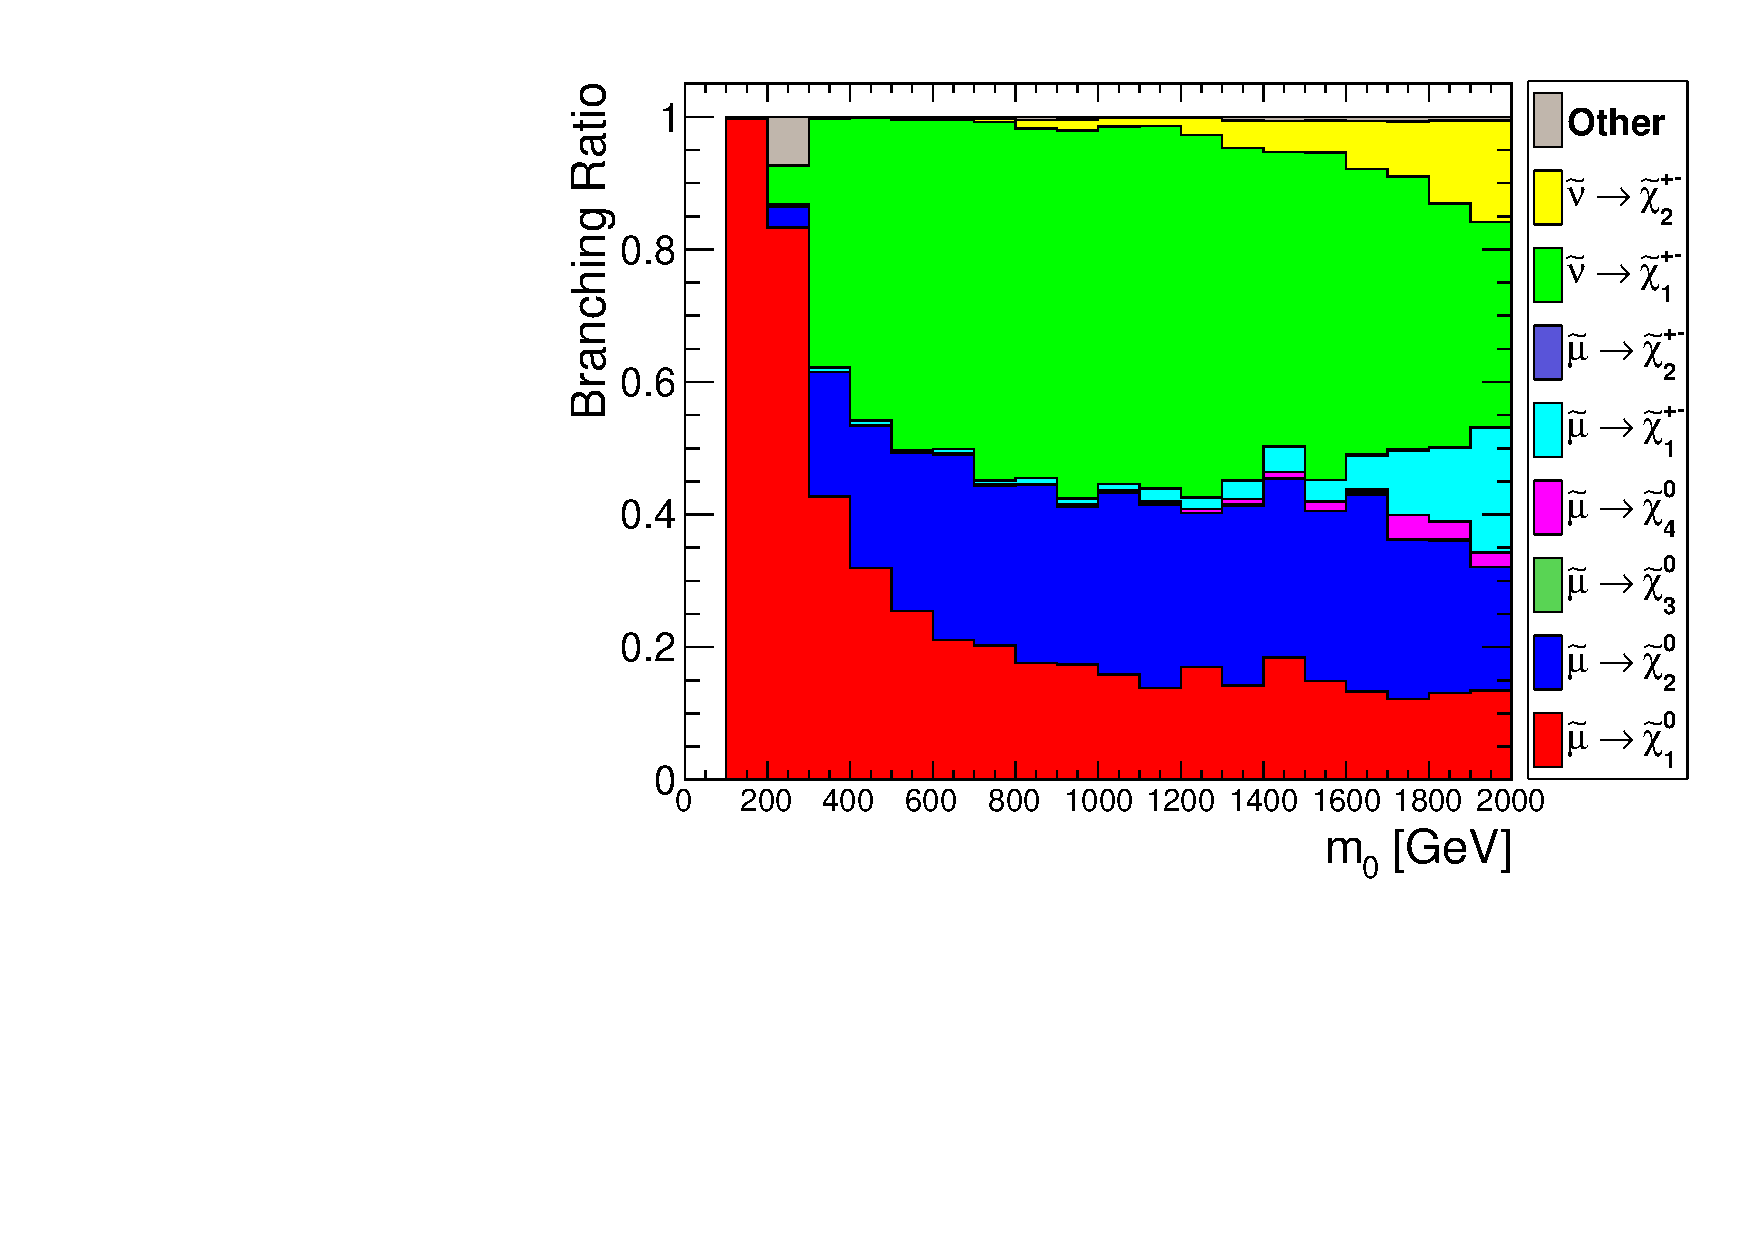
\includegraphics[width=\textwidth]{plots/hCutCrossRatio550.pdf}
    \caption{$m_{1/2} = 550\,\text{GeV}$\label{fig:cutcrossratio550}}
  \end{subfigure}

  \begin{subfigure}[b]{0.495\textwidth}
    \centering
    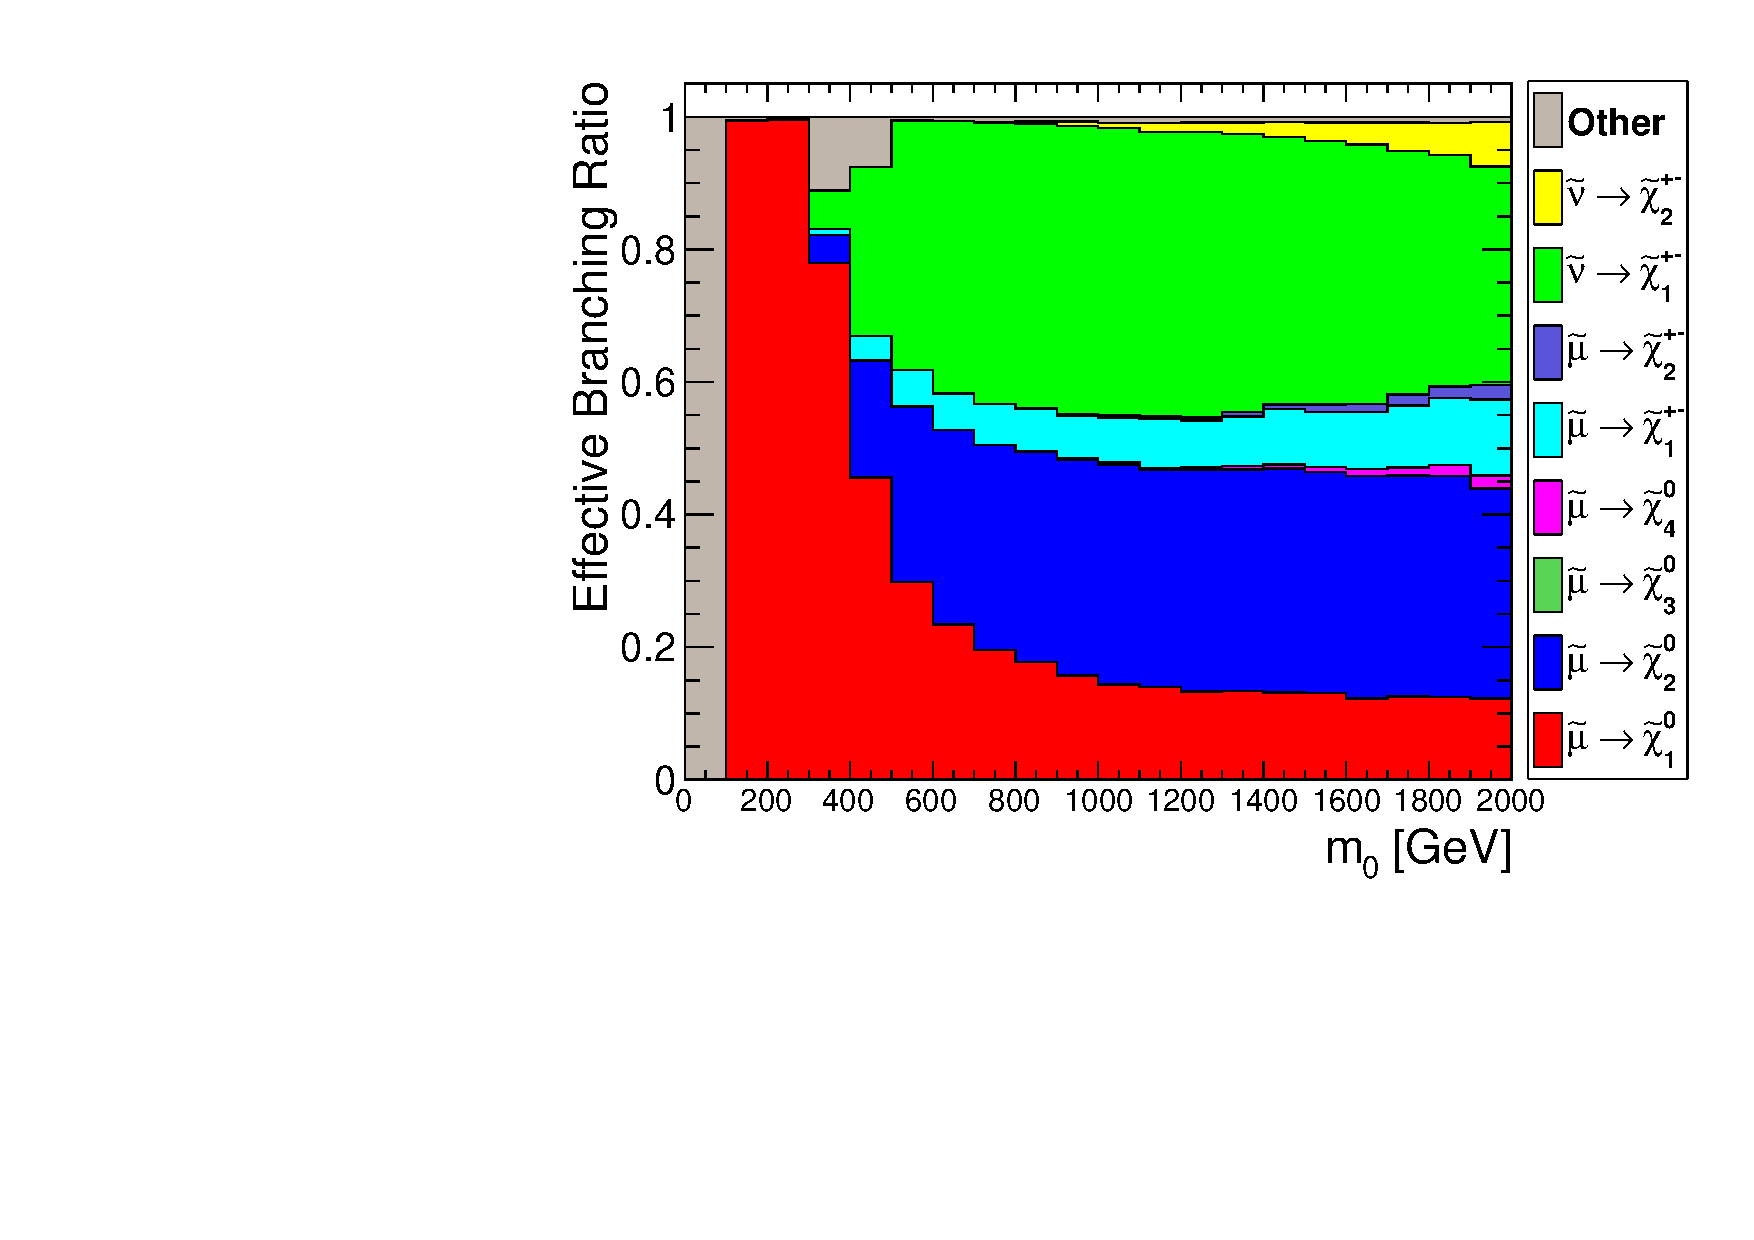
\includegraphics[width=\textwidth]{plots/hCrossRatio750.pdf}
    \caption{$m_{1/2} = 750\,\text{GeV}$\label{fig:crossratio750}}
  \end{subfigure}
  \begin{subfigure}[b]{0.495\textwidth}
    \centering
    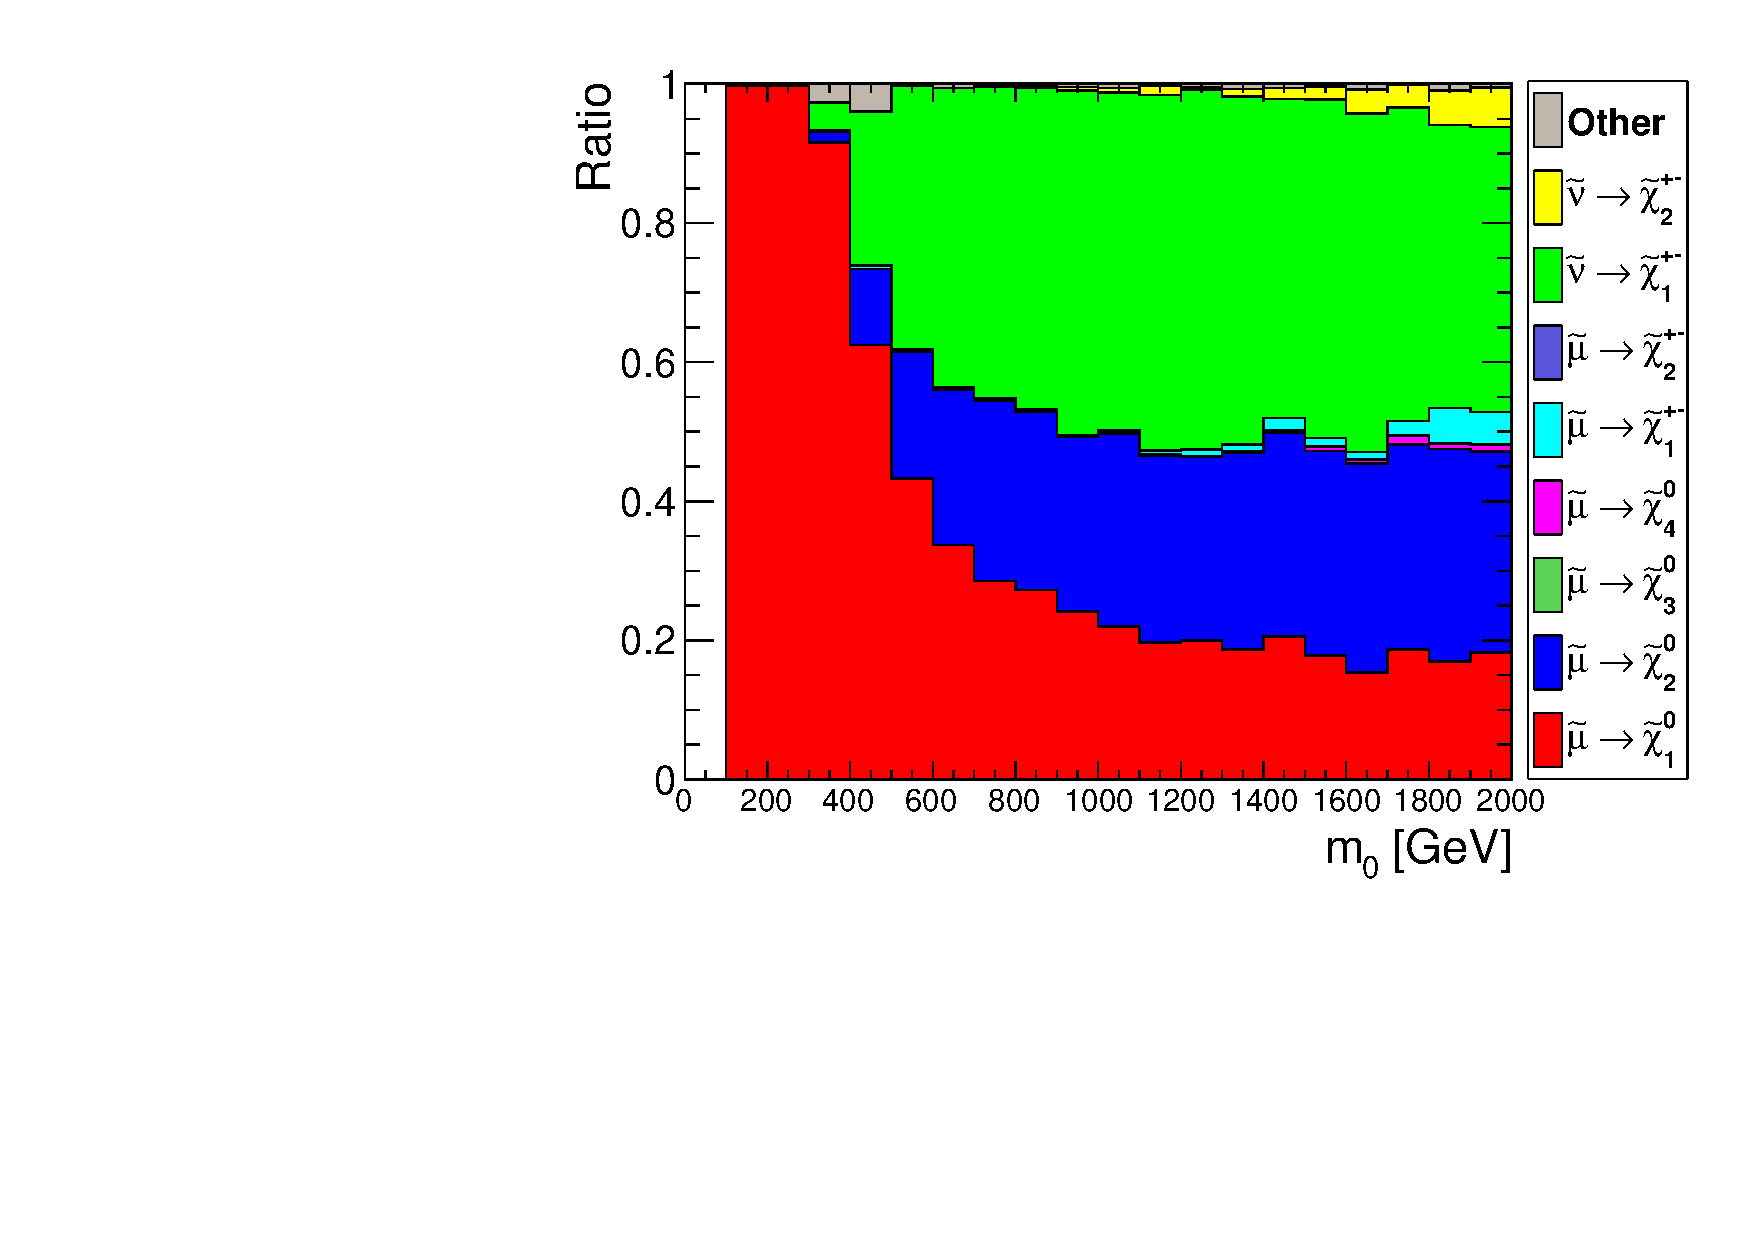
\includegraphics[width=\textwidth]{plots/hCutCrossRatio750.pdf}
    \caption{$m_{1/2} = 750\,\text{GeV}$\label{fig:cutcrossratio750}}
  \end{subfigure}

  \caption{Sum of all ERBs for the events from figure~\ref{fig:sigeff} for fixed values of $m_{1/2}$. All distributions on the left show the MU2J2 case, while the ANA case is given on the right side. Each color represents the ERB from a different process.}
  \label{fig:crossratios}
\end{figure}

Taking the empty bins into account (Cf.~\ref{fig:sigeff}), $550\,\text{GeV}$ as a value for $m_{1/2}$ provides a reasonable overview shown in figures~\ref{fig:crossratio550} and \ref{fig:cutcrossratio550}. To ensure a similar behaviour over the entire $m_{1/2}$ range, two variations with a $200\,\text{GeV}$ difference in the value of $m_{1/2}$ are used for confirmation (Fig.~\ref{fig:crossratio350},~\ref{fig:cutcrossratio350},~\ref{fig:crossratio750} and \ref{fig:cutcrossratio750}). With the grey colour marking the remaining contribution, only a negligible part of the total EBR is not covered by the listed processes. Initially, this statement would contradict the first bin of the MU2J2 case. However, since a \textit{ratio} is being shown, this can be explained by the very low number of selected events in this region (Cf.~\ref{fig:sigeff}). The ANA case supports this explanation, as none of the events pass its requirements.

As one would expect, for higher sfermion masses the contribution from processes with heavier sparticles increases. However the conclusion that can be drawn from these distributions, is that three processes dominate the signature of this analysis' signal. This is only enhanced by transitioning from the MU2J2, to the ANA case. The corresponding Feynman graphs for the three processes are given in figure~\ref{fig:domprocesses}.

\begin{figure}[htb!]
  \centering
  \begin{subfigure}[b]{0.495\textwidth}
    \centering
    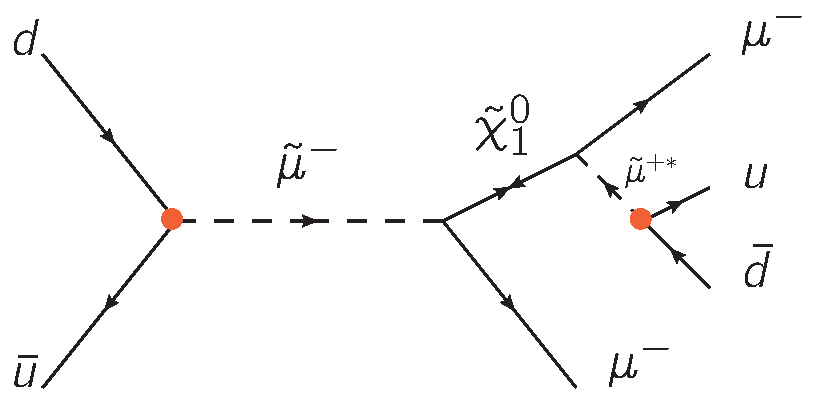
\includegraphics[width=\textwidth]{plots/rpv-resonant-smuon-samesign-mumuqq.pdf}
    \caption{\label{fig:resosmuneut1}}
  \end{subfigure}
  \begin{subfigure}[b]{0.495\textwidth}
    \centering
    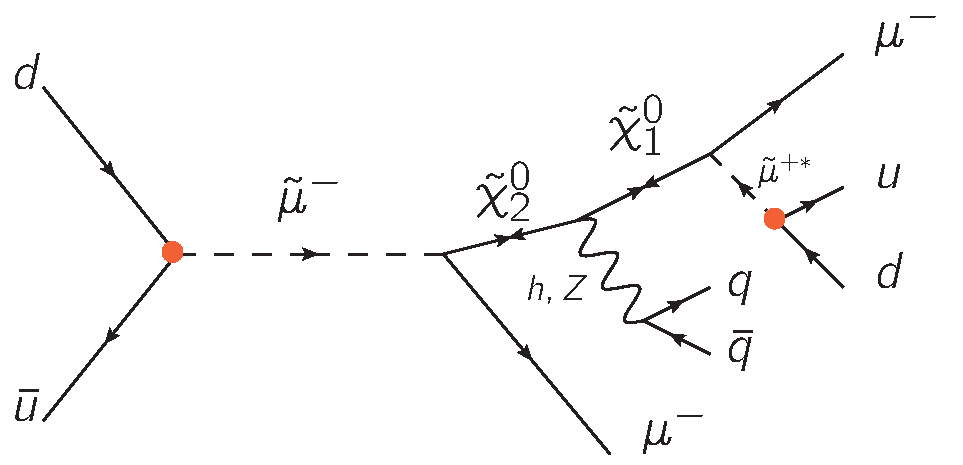
\includegraphics[width=\textwidth]{plots/rpv-resonant-smuon-neutralino2.pdf}
    \caption{\label{fig:resosmuneut2}}
  \end{subfigure}

  \begin{subfigure}[b]{0.495\textwidth}
    \centering
    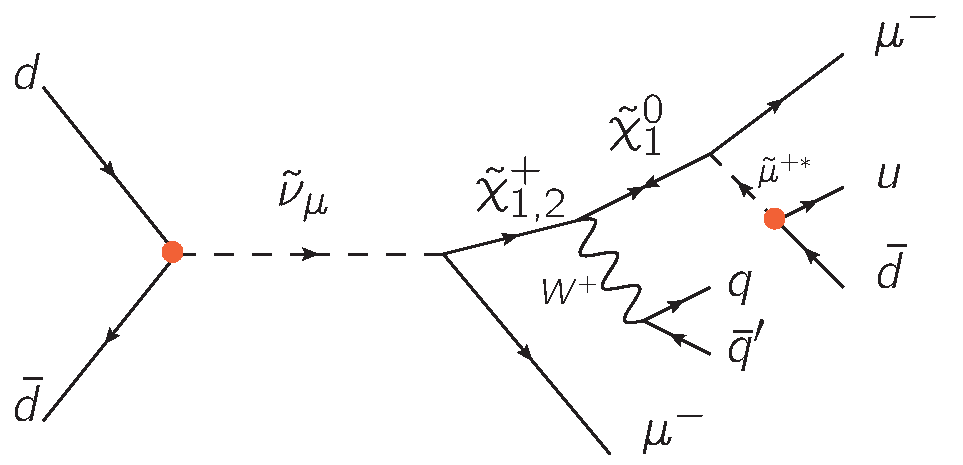
\includegraphics[width=\textwidth]{plots/rpv-resonant-sneutrino-chargino-mumuqq.pdf}
    \caption{\label{fig:resosneutcharg1}}
  \end{subfigure}

  \caption{Feynman graphs of the three dominant processes that lead to the signal signature. Each of the cascades leads to the neutralino LSP, which then decays through the $\lambda^\prime_{211}$ coupling, adding two jets and one muon to the final state.}
  \label{fig:domprocesses}
\end{figure}

\noindent As mentioned beforehand, after reaching the LSP through the cascade, the decay through the $\lambda^\prime_{211}$ leading to two jets and one muon is identical for every process. The simplest graph (Fig.~\ref{fig:resosmuneut1}) has its biggest contribution of up to almost $100\pct$ in the low $m_0$ region. It then quickly loses importance and remains at a constant level around $20\pct$. Both the other processes gain importance as the simple one loses it. Their contribution levels around $25\pct$ for the $\tilde{\mu} \rightarrow \tilde{\chi}^0_2$ and $45\pct$ for the $\tilde{\nu} \rightarrow \tilde{\chi}^\pm_1$ process for $500\,\text{GeV} < m_0 < 1600\,\text{GeV}$. Afterwards they decrease slowly.

This information can be used to allow for different interpretations of the results of this analysis. In addition to using the supersymmetric model, simplified models for the three Feynman graphs are an option. Since these types of models only focus on the physical parameters such as the particle mass and coupling strengths, it is easier to interpret these results for other models.



%%% Local Variables: 
%%% mode: latex
%%% TeX-master: "document"
%%% End: 
